% Options for packages loaded elsewhere
\PassOptionsToPackage{unicode}{hyperref}
\PassOptionsToPackage{hyphens}{url}
%
\documentclass[
]{article}
\usepackage{amsmath,amssymb}
\usepackage{lmodern}
\usepackage{iftex}
\ifPDFTeX
  \usepackage[T1]{fontenc}
  \usepackage[utf8]{inputenc}
  \usepackage{textcomp} % provide euro and other symbols
\else % if luatex or xetex
  \usepackage{unicode-math}
  \defaultfontfeatures{Scale=MatchLowercase}
  \defaultfontfeatures[\rmfamily]{Ligatures=TeX,Scale=1}
\fi
% Use upquote if available, for straight quotes in verbatim environments
\IfFileExists{upquote.sty}{\usepackage{upquote}}{}
\IfFileExists{microtype.sty}{% use microtype if available
  \usepackage[]{microtype}
  \UseMicrotypeSet[protrusion]{basicmath} % disable protrusion for tt fonts
}{}
\makeatletter
\@ifundefined{KOMAClassName}{% if non-KOMA class
  \IfFileExists{parskip.sty}{%
    \usepackage{parskip}
  }{% else
    \setlength{\parindent}{0pt}
    \setlength{\parskip}{6pt plus 2pt minus 1pt}}
}{% if KOMA class
  \KOMAoptions{parskip=half}}
\makeatother
\usepackage{xcolor}
\usepackage{longtable,booktabs,array}
\usepackage{calc} % for calculating minipage widths
% Correct order of tables after \paragraph or \subparagraph
\usepackage{etoolbox}
\makeatletter
\patchcmd\longtable{\par}{\if@noskipsec\mbox{}\fi\par}{}{}
\makeatother
% Allow footnotes in longtable head/foot
\IfFileExists{footnotehyper.sty}{\usepackage{footnotehyper}}{\usepackage{footnote}}
\makesavenoteenv{longtable}
\setlength{\emergencystretch}{3em} % prevent overfull lines
\providecommand{\tightlist}{%
  \setlength{\itemsep}{0pt}\setlength{\parskip}{0pt}}
\setcounter{secnumdepth}{-\maxdimen} % remove section numbering
\usepackage[margin=1.1in]{geometry}
\usepackage{graphicx}
\usepackage{float}
\usepackage{placeins}
\usepackage[table]{xcolor}
\definecolor{amber}{RGB}{255,191,0}
\definecolor{greenpoint}{RGB}{0,120,0}
\definecolor{bluepoint}{RGB}{30,90,180}
\ifLuaTeX
  \usepackage{selnolig}  % disable illegal ligatures
\fi
\IfFileExists{bookmark.sty}{\usepackage{bookmark}}{\usepackage{hyperref}}
\IfFileExists{xurl.sty}{\usepackage{xurl}}{} % add URL line breaks if available
\urlstyle{same} % disable monospaced font for URLs
\hypersetup{
  hidelinks,
  pdfcreator={LaTeX via pandoc}}

\author{}
\date{}

\begin{document}

\begin{titlepage}
\centering

{\Huge What Linguistic Features Differentiate High-Engagement and Low-Engagement Online Reviews? Evidence from Yelp Restaurant Reviews\par}

\vspace{1.5cm}

{\Large
Alexander Shan \\
\vspace{0.1cm}
Texas Academy of Mathematics and Science \\
\vspace{0.5cm}
Angela Yin \\
\vspace{0.1cm}
Reedy High School
}

\vspace{1.5cm}

{\large August 2026}

\vfill

{\small
Correspondence: \\
Alexander Shan - alsney2019@gmail.com \\
Angela Yin - angelasuyuyin@gmail.com 
}

\vspace{0.5cm}

\end{titlepage}

\fontsize{12pt}{12pt}\selectfont

\hypertarget{abstract}{%
\section{Abstract}\label{abstract}}

Online reviews influence how people choose restaurants and other
services, and engagement levels on Yelp vary substantially across
reviews. This study analyzes a large sample of Yelp restaurant reviews
and extracts linguistic features covering sentiment, lexical diversity,
readability, syntactic structure, and formatting. Logistic Regression
and XGBoost models are trained to distinguish reviews that received
engagement votes from those that received none, with both models
reaching test AUC values near 0.71. SHAP analysis identifies review
length, vocabulary size, syntactic depth, and punctuation patterns as
the most influential features. A temporal comparison shows that reviews
from two older periods exhibit a similar feature‑importance pattern,
indicating that the associations are stable after controlling for
exposure‑time differences. Because engagement also reflects visibility
and platform dynamics, the results represent associations rather than
causal effects, but they point to consistent linguistic characteristics
linked to higher reader interaction in this dataset.

\hypertarget{introduction}{%
\section{1. Introduction}\label{introduction}}

Online reviews shape everyday decisions, from choosing a restaurant to
booking a hotel. Platforms like Yelp host millions of reviews, and
engagement levels vary widely across them, reflected in votes such as
``useful,'' ``funny,'' or ``cool.'' Understanding why certain reviews
draw attention while others do not is important for both readers and
platforms that rely on user‑generated content.

Much of the existing research on online reviews focuses on detecting
deception, but the Yelp Open Dataset does not include labels that
identify whether a review is fake. Rather than trying to infer deception
without ground‑truth data, this study looks at a different question:
whether aspects of writing style can help explain which reviews readers
respond to and find helpful.

This study asks a central question:

\emph{Can linguistic - features such as vocabulary richness,
readability, sentiment, and syntactic structure - predict whether a Yelp
review receives engagement from other users?}

To investigate this question, we analyze Yelp restaurant reviews using a
structured set of linguistic features and two machine‑learning models.
Engagement votes serve as a practical, review‑level indicator of
perceived helpfulness. The goal is not simply to build predictive
models, but to identify the linguistic patterns that distinguish
high‑engagement reviews from those that receive no votes. These analyses
identify which aspects of writing style are associated with higher
engagement in this dataset. Understanding these associations is useful
for both writers, who often want their reviews to be noticed, and
platforms, which need additional signals when engagement votes are
sparse. Because many reviews receive no votes, linguistic features offer
platforms another way to identify reviews that may be helpful when
direct engagement signals are missing.

In this study, the machine‑learning models are used as tools to
highlight which linguistic features matter most. The focus is on writing
style and its relationship to engagement, not on comparing model
performance.

\hypertarget{related-work}{%
\section{2. Related Work}\label{related-work}}

Research on online review quality spans three major areas:

\begin{itemize}

\item \textbf{Deception detection —}  
Early work (Jindal \& Liu, 2008; Mihalcea \& Strapparava, 2009; Ott et al., 2011) examined linguistic cues associated with fake reviews, later incorporating syntactic stylometry (Feng et al., 2012) and behavioral metadata (Mukherjee et al., 2013). Although neural and transformer‑based text models have become standard tools for document classification, recent advances in review analysis have focused more on helpfulness and engagement prediction than on deception. Because Yelp’s Open Dataset does not include filtered reviews or ground‑truth deception labels, these methods cannot be directly applied here.

\item \textbf{Helpfulness prediction —}  
Foundational studies on Amazon (Kim et al., 2006; Ghose \& Ipeirotis, 2011) show that crowd‑sourced helpfulness votes correlate with linguistic properties such as sentiment, specificity, readability, and emotional tone. More recent work extends these findings using neural architectures: Qu et al. (2020) introduce an attention‑based model that incorporates customer‑expectation signals, Du et al. (2021) propose a neighbor‑aware framework that leverages relational information among reviews, and Saumya \& Kumar (2023) provide a comprehensive survey of modern deep‑learning approaches to helpfulness prediction.

\item \textbf{Linguistic and stylistic analysis —}  
A broader line of work investigates stylistic markers including part‑of‑speech patterns, syntactic complexity, vocabulary richness, and other structural indicators of writing quality. Contemporary neural models also incorporate these features: the helpfulness‑prediction approaches discussed above (e.g., Qu et al., 2020; Du et al., 2021) explicitly leverage linguistic cues within attention‑based and relational architectures. Survey work (Saumya \& Kumar, 2023) further highlights that interpretable linguistic features remain influential even as review‑quality modeling shifts toward deep learning.

\end{itemize}

This study aligns most closely with helpfulness‑prediction and
engagement‑modeling research, but differs by using interpretable
linguistic features to identify the textual characteristics associated
with Yelp review engagement. Because Yelp does not provide deception
labels, the focus remains on linguistic signals of perceived reliability
rather than on detecting fraudulent content.

\hypertarget{dataset}{%
\section{3. Dataset}\label{dataset}}

\hypertarget{overview}{%
\subsection{3.1 Overview}\label{overview}}

The Yelp Open Dataset is distributed across several structured JSON
files, each capturing a different aspect of the platform's ecosystem.
The \textbf{business} file contains location data, attributes, and
category metadata for each business. The \textbf{review} file provides
full review text along with user and business identifiers. The
\textbf{user} file includes user‑level metadata such as friend mappings
and account attributes. The \textbf{checkin} file records check‑in
activity for businesses, while the \textbf{tip} file contains short
user‑written suggestions that complement full reviews. Although the
dataset also includes a \textbf{photo} file, which stores image captions
and classifications (e.g., ``food,'' ``menu,'' ``inside''), these
auxiliary files are not used for this study. Only the business and
review files are used, as they provide all necessary information for
domain filtering, linguistic feature extraction, and engagement
labeling.

Each review includes full text, a star rating, a timestamp and
engagement metrics (useful, funny, cool) contributed by other users.
These engagement signals serve as non-linguistic, crowd-sourced
indicators of perceived helpfulness.

To reduce domain-driven variation, this study focuses exclusively on
restaurant reviews. The data-processing pipeline proceeds as follows:

\begin{itemize}  

\item Identify restaurant businesses by filtering the business file using category keywords.
\item Merge the business and review files to retain only reviews associated with restaurant businesses.
\item Apply a 5\% random sample to the restaurant reviews to create a tractable subset for NLP feature extraction.
\item Compute linguistic features on the sampled reviews, including lexical, structural, syntactic, and stylistic indicators.
\item Construct engagement labels (High, Low, Intermediate) to finalize the modeling dataset.

\end{itemize}

Applying this pipeline yields 5,245,324 restaurant reviews that meet the
filtering criteria. From this set, a 5\% random sample is drawn,
producing 261,882 reviews for feature engineering and subsequent
analysis. This sampled subset is large enough to support robust
descriptive comparisons and predictive modeling. After linguistic
feature extraction, the reviews are categorized into high‑, low‑, and
intermediate‑engagement groups, forming the final labeled dataset used
throughout the study. Together, these steps produce a domain‑consistent,
computationally manageable dataset that is fully annotated with both
linguistic features and engagement labels.

Because engagement votes accumulate over time, newer reviews may appear
low‑engagement simply because they have had less opportunity to receive
votes. To account for this exposure‑time bias, we conduct a temporal
segmentation analysis to examine whether the linguistic patterns
identified in our study remain stable across different temporal periods.
The results show that the influential features persist among older
reviews and partially persist in the most recent reviews, indicating
that the main drivers of high engagement are largely the identified
linguistic features rather than differences in exposure time.

\hypertarget{sampling}{%
\subsection{3.2 Sampling}\label{sampling}}

Although the Yelp Open Dataset contains millions of restaurant reviews,
analyzing the full corpus is computationally unnecessary for the goals
of this study. A 5\% random sample of the filtered restaurant‑review set
(261,882 reviews) is used to balance computational efficiency with
statistical power. Random sampling preserves variation in review length,
diversity in writing style, distribution of star ratings, and the
natural frequency of engagement signals, ensuring that linguistic
patterns observed in the sample generalize to the broader population of
Yelp restaurant reviews. The 5\% sampling rate was selected to make the
feature‑engineering stage computationally manageable. Generating
linguistic features for millions of reviews requires substantial
processing time, especially when using NLP tools such as spaCy and
textstat on a standard home computer. Several sampling percentages were
tested, and 5\% provided a practical balance: the resulting dataset of
over 260,000 reviews is large enough to preserve linguistic diversity
and support reliable analysis, while keeping preprocessing and feature
extraction within a reasonable runtime of a few hours.

\hypertarget{label-construction}{%
\subsection{3.3 Label Construction}\label{label-construction}}

The Yelp Open Dataset does not provide an explicit engagement label, so
we construct one using the three available engagement fields: useful,
funny, and cool. Reviews are assigned to High‑, Low‑, or
Intermediate‑engagement categories based on the following criteria:

\begin{itemize}  
\item \textbf{High-engagement}: useful >= 2 OR funny >= 1 OR cool >= 1
\item \textbf{Low-engagement}: useful = 0 AND funny = 0 AND cool = 0  
\item \textbf{Intermediate}: all remaining cases  
\end{itemize}

These categories capture how other users responded to a review and serve
as a proxy for perceived helpfulness. The thresholds are chosen to
separate reviews that received clear, non‑trivial engagement from those
that received none. A cutoff of two ``useful'' votes reduces noise from
single‑vote cases, which often reflect minimal or incidental
interaction. In contrast, ``funny'' and ``cool'' votes occur less
frequently overall, so a threshold of one is sufficient to indicate
meaningful attention. The asymmetric thresholds therefore reflect the
different usage patterns of the three engagement signals and produce a
more stable distinction between high‑ and low‑engagement reviews.
Intermediate cases are excluded because their engagement levels are
ambiguous and do not provide a clear contrast for modeling.

\hypertarget{traintest-split-for-modeling}{%
\subsection{3.4 Train--Test Split for
Modeling}\label{traintest-split-for-modeling}}

After constructing the labeled restaurant‑review dataset, an 80/20
train--test split is applied to support predictive modeling. The
training set is used to fit all models, while the held‑out test set
provides an unbiased estimate of predictive performance and supports
SHAP‑based interpretability analysis.

\hypertarget{methodology}{%
\section{4. Methodology}\label{methodology}}

This study investigates whether linguistic features can distinguish
high-engagement from low-engagement Yelp reviews. The methodology
integrates standardized text preprocessing, structured linguistic
feature engineering, and interpretable machine-learning models, all
applied within the restaurant review domain to maintain linguistic
consistency and avoid cross‑domain confounds.

\hypertarget{preprocessing}{%
\subsection{4.1 Preprocessing}\label{preprocessing}}

A minimal preprocessing pipeline is applied to all review text to ensure
consistency while preserving the full linguistic structure required for
feature extraction. Each review is lowercased, stripped of leading and
trailing whitespace, and normalized so that repeated whitespace is
collapsed into a single space. No punctuation or stop words are removed,
and no additional text transformations are applied. The normalized text
is then passed directly into spaCy, and all linguistic
features---lexical, syntactic, readability, structural, sentiment, and
semantic---are computed from the resulting document.

\hypertarget{linguistic-feature-engineering}{%
\subsection{4.2 Linguistic Feature
Engineering}\label{linguistic-feature-engineering}}

Linguistic features are extracted to capture multiple dimensions of
writing style, emotional tone, and textual complexity. All features are
computed from the same spaCy document produced by the preprocessing step
in Section 4.1. Feature-specific filtering is applied within the
extraction process to isolate the relevant linguistic signals. For
example, lexical features use alphabetic tokens and their lemmas, while
syntactic, readability, structural, sentiment, and semantic features
rely on the full document, including punctuation and stop words.

Feature extraction is implemented using spaCy for tokenization,
lemmatization, part-of-speech tagging, and dependency parsing; textstat
for readability metrics; and VADER for sentiment scoring. The resulting
feature set spans six interpretable categories---lexical, syntactic,
readability, sentiment, structural, and semantic---providing a
comprehensive representation of each review's linguistic
characteristics.

\textbf{Table 4.1: Lexical Features}

\begin{longtable}[]{@{}
  >{\raggedright\arraybackslash}p{(\columnwidth - 2\tabcolsep) * \real{0.2676}}
  >{\raggedright\arraybackslash}p{(\columnwidth - 2\tabcolsep) * \real{0.7324}}@{}}
\toprule()
\begin{minipage}[b]{\linewidth}\raggedright
Feature
\end{minipage} & \begin{minipage}[b]{\linewidth}\raggedright
Description
\end{minipage} \\
\midrule()
\endhead
token\_count & Number of alphabetic tokens in the text \\
unique\_tokens & Count of distinct surface word forms \\
unique\_lemmas & Count of distinct lemmas (vocabulary size) \\
type\_lemma\_ratio & Unique lemmas divided by total tokens; lemma-based
diversity \\
avg\_word\_len & Average number of characters per word \\
hapax\_ratio & Fraction of lemmas appearing exactly once \\
\bottomrule()
\end{longtable}

\textbf{Table 4.2: Syntactic Features}

\begin{longtable}[]{@{}
  >{\raggedright\arraybackslash}p{(\columnwidth - 2\tabcolsep) * \real{0.2615}}
  >{\raggedright\arraybackslash}p{(\columnwidth - 2\tabcolsep) * \real{0.7385}}@{}}
\toprule()
\begin{minipage}[b]{\linewidth}\raggedright
Feature
\end{minipage} & \begin{minipage}[b]{\linewidth}\raggedright
Description
\end{minipage} \\
\midrule()
\endhead
noun\_count & Number of nouns; concreteness indicator \\
verb\_count & Number of verbs; action orientation \\
adj\_count & Number of adjectives; descriptiveness \\
adv\_count & Number of adverbs; modifier intensity \\
avg\_dep\_depth & Average syntactic dependency chain length;
complexity \\
\bottomrule()
\end{longtable}

\textbf{Table 4.3: Readability Features}

\begin{longtable}[]{@{}
  >{\raggedright\arraybackslash}p{(\columnwidth - 2\tabcolsep) * \real{0.2614}}
  >{\raggedright\arraybackslash}p{(\columnwidth - 2\tabcolsep) * \real{0.7386}}@{}}
\toprule()
\begin{minipage}[b]{\linewidth}\raggedright
Feature
\end{minipage} & \begin{minipage}[b]{\linewidth}\raggedright
Description
\end{minipage} \\
\midrule()
\endhead
flesch\_reading\_ease & Standard readability score; higher = easier \\
smog\_index & Readability index based on polysyllabic words \\
ari & Automated Readability Index; character-based difficulty \\
coleman\_liau & Readability score using characters per word and words
per sentence \\
dale\_chall & Readability score based on proportion of ``hard'' words \\
\bottomrule()
\end{longtable}

Readability metrics are included to capture surface‑level aspects of
writing complexity that may influence how readers process a review.
These features complement the lexical and syntactic measures by
providing an additional perspective on how easily a review can be read.
Including readability scores ensures that the feature set covers
multiple dimensions of writing style, allowing later analyses to
determine which aspects are most relevant to engagement.

\textbf{Table 4.4: Sentiment Features}

\begin{longtable}[]{@{}
  >{\raggedright\arraybackslash}p{(\columnwidth - 2\tabcolsep) * \real{0.2644}}
  >{\raggedright\arraybackslash}p{(\columnwidth - 2\tabcolsep) * \real{0.7356}}@{}}
\toprule()
\begin{minipage}[b]{\linewidth}\raggedright
Feature
\end{minipage} & \begin{minipage}[b]{\linewidth}\raggedright
Description
\end{minipage} \\
\midrule()
\endhead
sentiment\_proxy & Heuristic polarity-based sentiment score \\
\bottomrule()
\end{longtable}

\textbf{Table 4.5: Structural Features}

\begin{longtable}[]{@{}
  >{\raggedright\arraybackslash}p{(\columnwidth - 2\tabcolsep) * \real{0.2703}}
  >{\raggedright\arraybackslash}p{(\columnwidth - 2\tabcolsep) * \real{0.7297}}@{}}
\toprule()
\begin{minipage}[b]{\linewidth}\raggedright
Feature
\end{minipage} & \begin{minipage}[b]{\linewidth}\raggedright
Description
\end{minipage} \\
\midrule()
\endhead
sent\_count & Number of sentences in the text \\
avg\_sent\_len & Average number of tokens per sentence \\
char\_count & Total number of characters \\
punctuation\_count & Number of punctuation marks \\
burstiness & Variance of sentence lengths; rhythm/pacing \\
\bottomrule()
\end{longtable}

\textbf{Table 4.6: Semantic Features}

\begin{longtable}[]{@{}
  >{\raggedright\arraybackslash}p{(\columnwidth - 2\tabcolsep) * \real{0.2676}}
  >{\raggedright\arraybackslash}p{(\columnwidth - 2\tabcolsep) * \real{0.7324}}@{}}
\toprule()
\begin{minipage}[b]{\linewidth}\raggedright
Feature
\end{minipage} & \begin{minipage}[b]{\linewidth}\raggedright
Description
\end{minipage} \\
\midrule()
\endhead
concreteness\_proxy & Nouns divided by tokens; concreteness indicator \\
action\_ratio & Verbs divided by tokens; action orientation \\
\bottomrule()
\end{longtable}

Several features in the tables may appear similar---for example,
counting nouns versus computing the proportion of nouns---but they
capture different aspects of language. Raw counts describe structural
properties of a review, while normalized ratios reflect meaning‑oriented
characteristics such as concreteness or action orientation. The feature
set was designed to capture observable aspects of writing style---such
as vocabulary variety, syntactic depth, readability, and
formatting---using measures that can be directly interpreted in terms of
linguistic behavior. We avoid representations that would be difficult to
explain in this context, such as high‑dimensional embeddings. These
features form the input to the models described in Section 4.3.

\hypertarget{models}{%
\subsection{4.3 Models}\label{models}}

This study uses two supervised learning models---Logistic Regression and
XGBoost---to evaluate whether linguistic features contain predictive
information about engagement. Although both models use the same feature
set, they differ in how they process input features and represent
relationships among them.

Logistic Regression provides a linear baseline with feature‑level
coefficients. Because the model optimizes a linear decision boundary,
all linguistic features are standardized using a StandardScaler prior to
training. Standardization ensures stable coefficient estimation and
allows the coefficients to reflect the relative influence of each
feature on the predicted probability that a review receives engagement.
Several structural and lexical features --- such as token count,
character count, sentence count, and unique lemma count --- are
naturally correlated because they all increase with review length.
Logistic Regression therefore distributes the underlying length signal
across multiple coefficients, which limits the extent to which
individual count‑based coefficients can be interpreted as independent
effects. In this study, Logistic Regression serves primarily as a linear
baseline and a directional check on feature influence, while XGBoost and
SHAP provide the main basis for fine‑grained attribution.

XGBoost is used to capture nonlinear relationships and interactions
among linguistic features. As a tree‑based ensemble method, it
determines splits based on the ordering of feature values rather than
their absolute magnitudes, so feature scaling is unnecessary. Operating
on raw features preserves natural variation and avoids superfluous
preprocessing. XGBoost also supports SHAP‑based interpretation, which
provides structured, sample‑level attributions for how individual
features influence predictions. SHAP, introduced by Lundberg \& Lee
(2017), offers a unified, model‑agnostic framework for computing
Shapley‑value explanations and enables transparent interpretation of
tree‑based models through the efficient TreeSHAP algorithm.

Model training is performed on reviews labeled as either high‑engagement
or low‑engagement; intermediate reviews are excluded as described in
Section\,5.1. After filtering, the dataset is split into training and
test sets using an 80/20 ratio. Although this reduces the size of the
modeling dataset relative to the original 5\% sample (261,882 reviews),
the resulting subsets remain sufficiently large for reliable estimation.

Hyperparameters for XGBoost are selected manually rather than through
automated tuning. The chosen configuration---300 trees, maximum depth of
6, learning rate of 0.05, and moderate subsampling and column
sampling---was identified through iterative experimentation and provides
stable performance without excessive model complexity. Extensive
hyperparameter optimization was not pursued because the primary goal is
to interpret how linguistic features relate to engagement rather than to
maximize predictive accuracy. Logistic Regression uses standard
regularization settings and serves as a baseline model.

Model performance is assessed using accuracy, precision, recall,
F1‑score, and area under the ROC curve (AUC), which provide a
comprehensive view of predictive effectiveness and enable comparison
between linear and nonlinear modeling approaches.

\hypertarget{model-interpretation}{%
\subsection{4.4 Model Interpretation}\label{model-interpretation}}

Interpretability is central to this study. Beyond evaluating predictive
accuracy, the goal is to understand \emph{which linguistic features most
strongly influence engagement} and \emph{whether these effects are
consistent across modeling approaches}. Because Logistic Regression and
XGBoost differ fundamentally in how they represent
relationships---linear coefficients versus nonlinear tree‑based
interactions---interpretation relies on model‑appropriate feature
\textbf{importance measures} and a rank‑based comparison framework.
These differences also interact with preprocessing: Logistic Regression
operates on standardized features, while XGBoost operates on raw,
unscaled features, which affects how importance values should be
interpreted.

\begin{itemize}

\item \textbf{Logistic Regression}  
Feature importance is derived from the magnitude and direction of model coefficients. Because the model is trained on standardized features, each coefficient reflects the change in engagement likelihood associated with a one–standard‑deviation increase in the corresponding linguistic feature. Positive coefficients indicate features associated with higher engagement likelihood, while negative coefficients indicate features associated with lower engagement. To ensure comparability across features, importance is assessed using the \textbf{absolute value} of coefficients, reflecting each feature’s overall influence regardless of direction. 

\item \textbf{XGBoost}  
Feature importance is evaluated using \textbf{SHAP}-based mean absolute contribution values. SHAP values quantify how much each raw (unscaled) feature contributes to predictions across all samples, capturing nonlinear effects, thresholding behavior, and interactions that Logistic Regression cannot represent. Because XGBoost is tree‑based and invariant to monotonic transformations, operating on unscaled features preserves natural feature structure and does not affect interpretability. SHAP values are computed using the TreeSHAP algorithm, which provides exact, efficient feature attributions for tree‑based models.

\end{itemize}

Because Logistic Regression coefficients and XGBoost SHAP values operate
on different scales---and arise from fundamentally different model
classes---raw magnitudes are not directly comparable. Instead,
importance is compared using \textbf{rank order}, providing a
model‑agnostic measure of relative influence across both linear and
nonlinear modeling approaches.

\hypertarget{results}{%
\section{5. Results}\label{results}}

\hypertarget{descriptive-linguistic-patterns}{%
\subsection{5.1 Descriptive Linguistic
Patterns}\label{descriptive-linguistic-patterns}}

We summarize the distribution of engagement labels by categorizing each
review into low‑engagement (0), intermediate (1), and high‑engagement
(2). Intermediate reviews are reported for completeness but excluded
from all modeling and interpretability analysis. All descriptive
statistics in later sections therefore reflect only the high‑ and
low‑engagement subsets.

\textbf{Table 5.1: Sample Overview}

\begin{longtable}[]{@{}llll@{}}
\toprule()
Engagement Category & Count & Percent & Included for modeling \\
\midrule()
\endhead
low-engagement & 134,436 & 51.3\% & 59.1\% \\
high-engagement & 93,007 & 35.5\% & 40.9\% \\
intermediate & 34,439 & 13.2\% & excluded \\
\textbf{Total} & 261,882 & 100.0\% & 100.0\% \\
\bottomrule()
\end{longtable}

\textbf{Table 5.2: Training and Test Sample Statistics}

\begin{longtable}[]{@{}llll@{}}
\toprule()
Sample & Engagement Category & Count & Percent \\
\midrule()
\endhead
Training & low-engagement & 107,549 & 59.1\% \\
& high-engagement & 74,405 & 40.9\% \\
Test & low-engagement & 26,887 & 59.1\% \\
& high-engagement & 18,602 & 40.9\% \\
\bottomrule()
\end{longtable}

With the dataset defined, we examine raw linguistic differences between
high‑ and low‑engagement reviews. Clear, systematic contrasts emerge
across lexical, structural, syntactic, and stylistic dimensions.

\begin{itemize}  

\item \textbf{High‑engagement reviews are substantially longer and content-rich}.  
They contain 311 more characters, 57 more tokens, 31 more unique tokens, and 29 more unique lemmas on average—each exceeding 50\% relative to the corresponding low‑engagement measures. These differences indicate that high‑engagement reviews provide more specific and elaborated content. Structural indicators reinforce this pattern: high‑engagement reviews include 3.66 additional sentences (57.61\%), exhibit longer average sentence length (11.70\%), and show higher burstiness (18.77\%), suggesting more developed narrative flow and greater topical elaboration.

\item \textbf{Syntactic features show strong divergence}.  
High‑engagement reviews use more nouns (+11.9), verbs (+7.3), adjectives (+4.9), and adverbs (+4.0)—each exceeding 50\% relative to the corresponding low‑engagement measures—reflecting denser descriptive content. Syntactic complexity increases as well: average dependency depth rises from 2.16 to 2.35 (8.85\%), indicating deeper syntactic structures and more elaborated phrasing.

\item \textbf{Stylistic markers point to greater expressive intensity}.  
High‑engagement reviews contain 8 additional punctuation marks, suggesting more emphasis, expressiveness, or rhetorical variation. Sentiment differences are modest but directionally consistent: the sentiment proxy increases from 0.68 to 0.70 (2.89\%), indicating a slightly more balanced or positive tone.

\item \textbf{Readability differences are small but directionally consistent}.  
High‑engagement reviews show slightly higher ARI, SMOG, and Dale–Chall scores, indicating marginally more complex writing. These shifts are minor compared to the pronounced structural, lexical, and syntactic contrasts observed above.

\end{itemize}

High‑engagement reviews are noticeably longer and contain more tokens,
which suggests that length may play an important role in how readers
respond to a review. However, length alone may not fully explain the
differences between the two groups. Although length is a meaningful
linguistic characteristic, many structural and lexical features scale
with review size, so part of their influence may reflect underlying
length differences rather than independent linguistic effects.

\textbf{Table 5.3: Mean Differences between Engagement Groups}

\begin{longtable}[]{@{}
  >{\raggedright\arraybackslash}p{(\columnwidth - 10\tabcolsep) * \real{0.1636}}
  >{\raggedright\arraybackslash}p{(\columnwidth - 10\tabcolsep) * \real{0.2909}}
  >{\raggedright\arraybackslash}p{(\columnwidth - 10\tabcolsep) * \real{0.1455}}
  >{\raggedright\arraybackslash}p{(\columnwidth - 10\tabcolsep) * \real{0.1455}}
  >{\raggedright\arraybackslash}p{(\columnwidth - 10\tabcolsep) * \real{0.1273}}
  >{\raggedright\arraybackslash}p{(\columnwidth - 10\tabcolsep) * \real{0.1273}}@{}}
\toprule()
\begin{minipage}[b]{\linewidth}\raggedright
Category
\end{minipage} & \begin{minipage}[b]{\linewidth}\raggedright
Feature
\end{minipage} & \begin{minipage}[b]{\linewidth}\raggedright
low engagement mean
\end{minipage} & \begin{minipage}[b]{\linewidth}\raggedright
high engagement mean
\end{minipage} & \begin{minipage}[b]{\linewidth}\raggedright
difference
\end{minipage} & \begin{minipage}[b]{\linewidth}\raggedright
pct diff
\end{minipage} \\
\midrule()
\endhead
Structural & char\_count & 412.07 & 723.79 & \textcolor{blue} {311.73} &
\textcolor{blue} {75.65\%} \\
Lexical & token\_count & 75.49 & 132.87 & \textcolor{blue} {57.38} &
\textcolor{blue} {76.02\%} \\
Lexical & unique\_tokens & 53.39 & 84.73 & \textcolor{blue} {31.34} &
\textcolor{blue} {58.71\%} \\
Lexical & unique\_lemmas & 50.64 & 79.60 & \textcolor{blue} {28.96} &
\textcolor{blue} {57.18\%} \\
Syntactic & noun\_count & 15.76 & 27.67 & \textcolor{blue} {11.90} &
\textcolor{blue} {75.51\%} \\
Structural & punctuation\_count & 10.30 & 18.45 &
\textcolor{blue} {8.16} & \textcolor{blue} {79.22\%} \\
Syntactic & verb\_count & 9.05 & 16.36 & \textcolor{blue} {7.31} &
\textcolor{blue} {80.70\%} \\
Syntactic & adj\_count & 7.93 & 12.85 & \textcolor{blue} {4.92} &
\textcolor{blue} {62.02\%} \\
Syntactic & adv\_count & 5.68 & 9.66 & \textcolor{blue} {3.99} &
\textcolor{blue} {70.27\%} \\
Structural & sent\_count & 6.36 & 10.02 & \textcolor{blue} {3.66} &
\textcolor{blue} {57.61\%} \\
Structural & avg\_sent\_len & 11.91 & 13.30 & 1.39 & 11.70\% \\
Structural & burstiness & 5.99 & 7.11 & 1.12 & 18.77\% \\
Readability & ari & 6.07 & 6.42 & 0.35 & 5.81\% \\
Readability & smog\_index & 8.73 & 8.95 & 0.22 & 2.56\% \\
Syntactic & avg\_dep\_depth & 2.16 & 2.35 & 0.19 & 8.85\% \\
Lexical & type\_lemma\_ratio & 0.76 & 0.68 & -0.07 & -9.82\% \\
Lexical & avg\_word\_len & 4.32 & 4.25 & -0.07 & -1.58\% \\
Lexical & hapax\_ratio & 0.81 & 0.77 & -0.04 & -5.07\% \\
Readability & dale\_chall & 8.01 & 8.05 & 0.04 & 0.47\% \\
Readability & coleman\_liau & 6.73 & 6.69 & -0.04 & -0.55\% \\
Sentiment & sentiment\_proxy & 0.68 & 0.70 & 0.02 & 2.89\% \\
Semantic & action\_ratio & 0.11 & 0.12 & 0.01 & 5.91\% \\
Semantic & concreteness\_proxy & 0.22 & 0.21 & -0.01 & -2.58\% \\
Readability & flesch\_reading\_ease & 74.96 & 74.96 & 0.00 & 0.00\% \\
\bottomrule()
\end{longtable}

\emph{All summary statistics in Table\,5.3 are computed on the full
dataset (training\,+\,test), whereas the tables in subsequent sections
report results using the held‑out test set only.}

\hypertarget{model-performance}{%
\subsection{5.2 Model Performance}\label{model-performance}}

To evaluate how well each model predicts whether a Yelp restaurant
review receives engagement, we report five standard classification
metrics. Each captures a different aspect of predictive behavior:

\begin{itemize}

\item \textbf{Accuracy -- } proportion of all predictions the model gets correct; reflects overall correctness.

\item \textbf{Precision --} among reviews predicted as high‑engagement, the fraction that truly are; measures false‑positive control.

\item \textbf{Recall -- } among all truly high‑engagement reviews, the fraction the model successfully identifies; measures false‑negative control.

\item \textbf{F1 Score -- } harmonic mean of precision and recall; balances the trade‑off between catching more positives and being correct when doing so.

\item \textbf{AUC -- } measures how well the model ranks reviews by engagement likelihood; higher values indicate better separation between classes.

\end{itemize}

With 41\% high‑engagement reviews, a majority‑class baseline still
yields an AUC of 0.5, so the models' AUC values around 0.705--0.706
represent substantial discriminative power from text alone.

\textbf{Table 5.4: Logistic Regressiion and XGB Model Performance}

\begin{longtable}[]{@{}
  >{\raggedright\arraybackslash}p{(\columnwidth - 10\tabcolsep) * \real{0.3188}}
  >{\raggedright\arraybackslash}p{(\columnwidth - 10\tabcolsep) * \real{0.1594}}
  >{\raggedright\arraybackslash}p{(\columnwidth - 10\tabcolsep) * \real{0.1449}}
  >{\raggedright\arraybackslash}p{(\columnwidth - 10\tabcolsep) * \real{0.1304}}
  >{\raggedright\arraybackslash}p{(\columnwidth - 10\tabcolsep) * \real{0.1304}}
  >{\raggedright\arraybackslash}p{(\columnwidth - 10\tabcolsep) * \real{0.1159}}@{}}
\toprule()
\begin{minipage}[b]{\linewidth}\raggedright
Model
\end{minipage} & \begin{minipage}[b]{\linewidth}\raggedright
Accuracy
\end{minipage} & \begin{minipage}[b]{\linewidth}\raggedright
Precision
\end{minipage} & \begin{minipage}[b]{\linewidth}\raggedright
Recall
\end{minipage} & \begin{minipage}[b]{\linewidth}\raggedright
F1 Score
\end{minipage} & \begin{minipage}[b]{\linewidth}\raggedright
\textbf{AUC}
\end{minipage} \\
\midrule()
\endhead
XGBoost & \textcolor{blue} {0.67080} & 0.63279 &
\textcolor{blue} {0.46457} & \textcolor{blue}{0.53579} &
\textcolor{blue}{0.70648} \\
Logistic Regression & 0.67054 & \textcolor{blue}{0.64299} & 0.43694 &
0.52031 & 0.70505 \\
\bottomrule()
\end{longtable}

To contextualize these results, we summarize the main performance
patterns observed across the two models:

\begin{itemize}

\item \textbf{Overall performance} - Both models achieve similar accuracy and AUC, indicating they capture the same underlying signals. 

\item \textbf{Logistic Regression} - Higher precision and lower recall, reflecting a more conservative boundary that flags fewer higher-engagement reviews but with greater accuracy.

\item \textbf{XGBoost} - Higher recall and lower precision, identifying more potentially engaging reviews while tolerating additional false positives due to its nonlinear model capacity.  

\item \textbf{F1 score} - XGBoost`s slightly higher F1 score shows a better precision-recall balance.

\item \textbf{Summary} - Performance is broadly similar, but XGBoost offers modest gains in detecting high-engagement reviews, whereas Logistic Regression provides more selective, precision-oriented predictions.  

\end{itemize}

\hypertarget{top-features-identified-by-xgboost}{%
\subsection{5.3 Top Features Identified by
XGBoost}\label{top-features-identified-by-xgboost}}

To identify the most influential predictors among the 24 linguistic
features, we classify the top one‑third of each model's ranked features
as its top‑tier set. This criterion provides a consistent basis for
determining which predictors each model considers most important.
Table\,5.5 summarizes these rankings: rank values that fall within the
top tier for either model are highlighted in blue, along with their mean
percentage differences from Section\,5.1.

XGBoost elevates eight features into its top‑tier group. These features
fall naturally into several interpretable linguistic categories:

\begin{itemize}

\item \textbf{Content richness and lexical sophistication:}  
unique lemmas (lexical richness), unique tokens (lexical diversity), type\_lemma\_ratio (lexical sophistication)

\item \textbf{Stylistic intensity:}  
punctuation count (stylistic emphasis)

\item \textbf{Review length:}  
character count (verbosity)

\item \textbf{Complexity and readability:}  
avg\_dep\_depth (syntactic complexity), avg\_word\_len (morphological complexity), flesch\_reading\_ease (readability)

\end{itemize}

This grouping highlights the dimensions XGBoost finds most predictive:
reviews that are lexically rich, stylistically expressive, sufficiently
detailed, and moderately complex and readable tend to receive more
engagement. Several of these features, such as character count and
punctuation count, also show clear mean differences between high‑ and
low‑engagement reviews, indicating that their importance aligns with
observable linguistic variation. Others, such as avg\_word\_len and
type\_lemma\_ratio, rise in importance because XGBoost captures
nonlinear interactions that amplify their predictive value.

\textbf{Table 5.5: Cross-Model Feature Importance Rank Comparison}

\begin{longtable}[]{@{}
  >{\raggedright\arraybackslash}p{(\columnwidth - 10\tabcolsep) * \real{0.1753}}
  >{\raggedright\arraybackslash}p{(\columnwidth - 10\tabcolsep) * \real{0.3608}}
  >{\raggedright\arraybackslash}p{(\columnwidth - 10\tabcolsep) * \real{0.1237}}
  >{\raggedright\arraybackslash}p{(\columnwidth - 10\tabcolsep) * \real{0.1340}}
  >{\raggedright\arraybackslash}p{(\columnwidth - 10\tabcolsep) * \real{0.0928}}
  >{\raggedright\arraybackslash}p{(\columnwidth - 10\tabcolsep) * \real{0.1134}}@{}}
\toprule()
\begin{minipage}[b]{\linewidth}\raggedright
Category
\end{minipage} & \begin{minipage}[b]{\linewidth}\raggedright
Feature
\end{minipage} & \begin{minipage}[b]{\linewidth}\raggedright
Abs Pct Diff
\end{minipage} & \begin{minipage}[b]{\linewidth}\raggedright
LR Coeff
\end{minipage} & \begin{minipage}[b]{\linewidth}\raggedright
LR Rank
\end{minipage} & \begin{minipage}[b]{\linewidth}\raggedright
SHAP Rank
\end{minipage} \\
\midrule()
\endhead
Lexical & \textbf{unique\_lemmas} & 57.18\% & 1.47 &
\textcolor{blue} {1} & \textcolor{blue} {1} \\
Lexical & \textbf{unique\_tokens} & 58.71\% & -0.07 & 10 &
\textcolor{blue} {3} \\
Lexical & \textbf{avg\_word\_len} & 1.58\% & -0.02 & 18 &
\textcolor{blue} {4} \\
Lexical & \textbf{type\_lemma\_ratio} & 9.82\% & -0.06 & 12 &
\textcolor{blue} {7} \\
Lexical & hapax\_ratio & 5.07\% & -0.06 & 11 & 12 \\
Lexical & token\_count & 76.02\% & 0.24 & \textcolor{blue} {5} & 21 \\
Syntactic & \textbf{avg\_dep\_depth} & 8.85\% & 0.10 &
\textcolor{blue} {6} & \textcolor{blue} {6} \\
Syntactic & noun\_count & 75.51\% & 0.04 & 13 & 15 \\
Syntactic & verb\_count & 80.70\% & -0.29 & \textcolor{blue} {4} & 18 \\
Syntactic & adj\_count & 62.02\% & -0.04 & 14 & 22 \\
Syntactic & adv\_count & 70.27\% & -0.01 & 24 & 23 \\
Readability & \textbf{flesch\_reading\_ease} & 0.003\% & 0.04 & 16 &
\textcolor{blue} {8} \\
Readability & dale\_chall & 0.47\% & 0.07 & 9 & 9 \\
Readability & coleman\_liau & 0.55\% & -0.01 & 21 & 13 \\
Readability & ari & 5.81\% & 0.02 & 19 & 14 \\
Readability & smog\_index & 2.56\% & -0.01 & 22 & 24 \\
Sentiment & sentiment\_proxy & 2.89\% & -0.03 & 17 & 10 \\
Structural & \textbf{punctuation\_count} & 79.22\% & 0.30 &
\textcolor{blue} {3} & \textcolor{blue} {2} \\
Structural & \textbf{char\_count} & 75.65\% & -1.11 &
\textcolor{blue} {2} & \textcolor{blue} {5} \\
Structural & avg\_sent\_len & 11.70\% & -0.04 & 15 & 11 \\
Structural & sent\_count & 57.61\% & 0.08 & \textcolor{blue} {7} & 16 \\
Structural & burstiness & 18.77\% & -0.02 & 20 & 20 \\
Semantic & action\_ratio & 5.91\% & 0.08 & \textcolor{blue} {8} & 17 \\
Semantic & concreteness\_proxy & 2.58\% & 0.01 & 23 & 19 \\
\bottomrule()
\end{longtable}

\hypertarget{cross-model-rank-agreement}{%
\subsection{5.4 Cross-Model Rank
Agreement}\label{cross-model-rank-agreement}}

To visualize the cross-model rank agreement, Figure\,5.1 plots each
feature's Logistic Regression rank against its XGBoost SHAP rank. The
resulting scatter plot shows a fair concentration of points along the
45‑degree diagonal, indicating areas of agreement, while the spread of
off‑diagonal points highlights where the two models diverge in their
feature rankings.

The color‑coded points in the figure further clarify the structure of
agreement and disagreement:

\begin{itemize}
\item \textcolor{greenpoint}{\textbf{Green}} points features ranked in the top eight by both models---cluster tightly near the diagonal and represent the strongest areas of cross‑model alignment.
\item \textcolor{bluepoint}{\textbf{Blue}} points show small deviations from the diagonal, reflecting modest rank differences and generally consistent behavior across models.
\item \textcolor{amber}{\textbf{Orange}} points sit farther from the diagonal, indicating moderate disagreement in how the models prioritize these features.
\item \textcolor{red}{\textbf{Red}} points notably token count, verb count, and avg\_word\_len---fall well outside the diagonal corridor and mark the largest rank discrepancies.
\end{itemize}

\FloatBarrier
\begin{figure}[H]
\centering
{\large \textbf{Figure 5.1: Cross-Model Feature Rank Comparison}}\

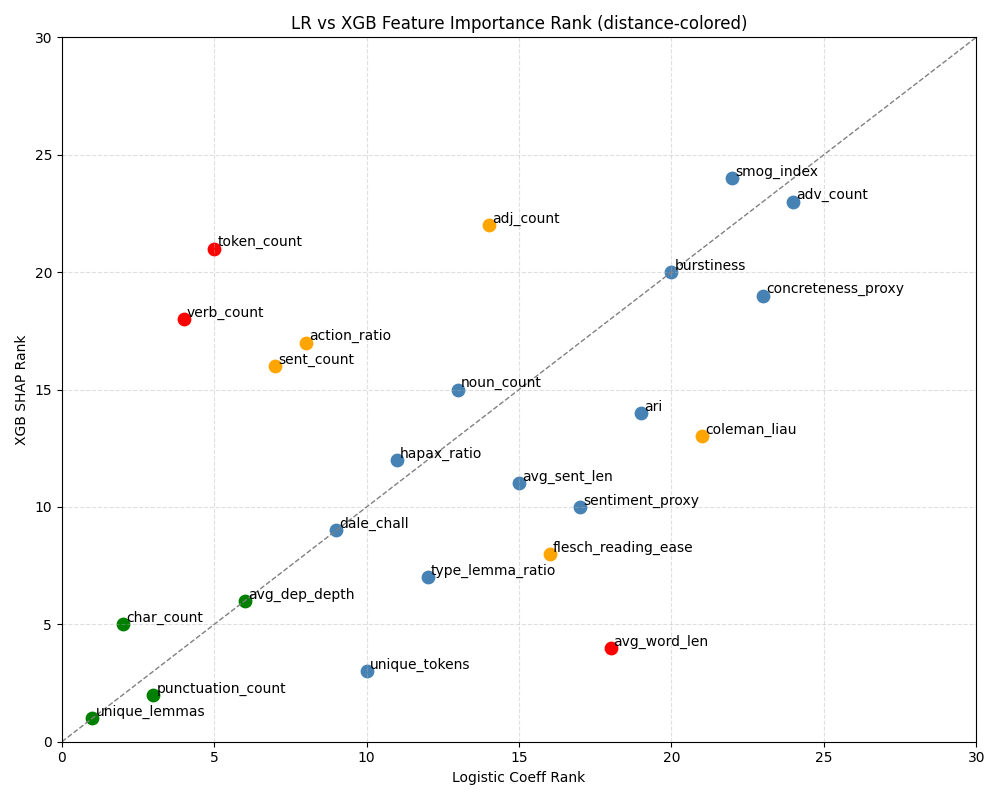
\includegraphics[width=1.05\textwidth]{fig_lr_shap_rank_distance_colored.png}
\label{fig:lr-shap-rank}
\end{figure}

\hypertarget{feature-effect-for-shared-top-features}{%
\subsection{5.5 Feature Effect for Shared Top
Features}\label{feature-effect-for-shared-top-features}}

To examine how the shared top features influence predictions, we compare
the marginal effects implied by both models for the four features they
jointly prioritize: unique lemmas, punctuation count, character count,
and avg\_dep\_depth. XGBoost's SHAP‑dependence plots and Logistic
Regression's \(X\beta\) contribution plots provide complementary views
of these effects. SHAP values capture nonlinear, context‑dependent
effects, while \(X\beta\) values represent strictly linear log‑odds
contributions. Because these arise from different modeling frameworks,
their y‑axes are not directly comparable, so we focus on the direction
and overall trend of each feature's effect rather than its absolute
magnitude.

\FloatBarrier
\begin{figure}[H]
\centering
{\large \textbf{Figure 5.2:  XGB SHAP Dependence Plot}}\

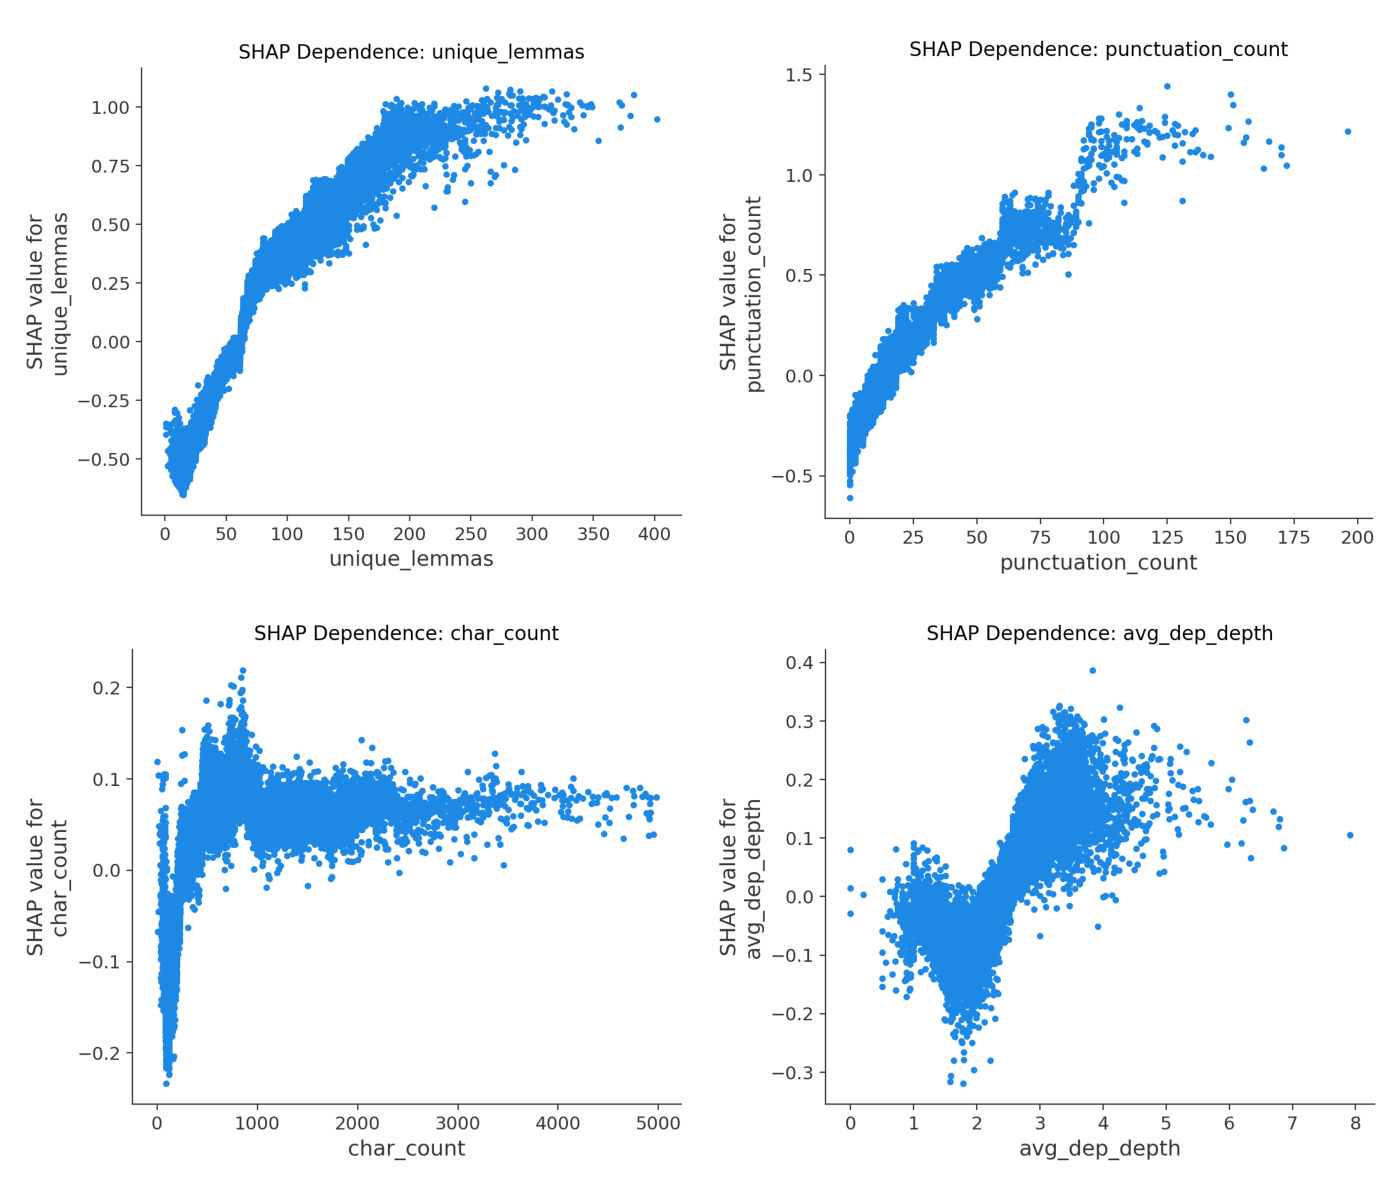
\includegraphics[width=1.05\textwidth]{05_xgb_top_features_shap_dependence.png}
\label{fig:xgb-shap-rank}
\end{figure}

\FloatBarrier
\begin{figure}[H]
\centering
{\large \textbf{Figure 5.3:  Logistic Regression XBETA Plot}}\

\includegraphics[width=1.05\textwidth]{05_lr_top_features_xbeta.png}
\label{fig:lr-xbeta}
\end{figure}

Across the four shared features, three show broadly similar directional
patterns, while one exhibits a clear difference:

\begin{itemize}

\item For \textbf{unique lemmas} and \textbf{punctuation count}, both models show positive contributions, with XGBoost capturing gentle curvature and Logistic Regression applying constant linear increases. 
\item For \textbf{character count}, the XGBoost SHAP dependence plot shows that the model assigns larger positive contributions to shorter reviews as length increases, after which the marginal effect levels off. This pattern reflects how the model uses character count in combination with correlated features such as token count, unique lemmas, and sentence count, rather than a causal threshold in review helpfulness.
\item For \textbf{avg\_dep\_depth}, the SHAP plot shows a similar leveling pattern: increases in dependency depth correspond to higher SHAP values up to a moderate range, after which the marginal contribution stabilizes. This behavior reflects the fitted model’s conditional associations and should not be interpreted as evidence that additional syntactic complexity becomes detrimental.

\end{itemize}

These plots illustrate how XGBoost models nonlinear associations among
correlated linguistic features, even though its overall predictive
performance is similar to the logistic model.

\hypertarget{feature-rank-stability-across-review-years}{%
\subsection{5.6 Feature Rank Stability Across Review
Years}\label{feature-rank-stability-across-review-years}}

Because Yelp reviews span 2005--2022 and the platform does not specify
when \emph{useful}, \emph{funny}, and \emph{cool} votes were last
aggregated, we treat engagement counts as a 2022 snapshot rather than
contemporaneous measurements. Older reviews have had many years to
accumulate validation, while newer reviews---especially those from
2019--2022---may not yet reflect their eventual engagement levels.
Ideally, engagement counts would be standardized to a fixed window
(e.g., two years after each review is written), but such information is
unavailable. To control for review age within the constraints of the
dataset, we segment the reviews into three balanced groups: Group\,1
(\(\le\)\,2015), Group\,2 (2016--2018), and Group\,3 (2019--2022),
containing 79,100, 80,999, and 67,344 reviews respectively.

The model is retrained within each segment, and segment‑specific SHAP
feature ranks are compared to the overall ranking. Figure\,5.4
summarizes these comparisons:

\begin{itemize}
\item
  Group\,1 (\(\le\)\,2015) --- Points lie close to the diagonal, showing
  strong alignment with the overall ranking.
\item
  Group\,2 (2016--2018) --- Similar tight clustering, indicating stable
  feature importance across mid‑period reviews.
\item
  Group\,3 (2019--2022) --- Wider spread and greater deviation from the
  diagonal, likely due to: limited time for recent reviews to accumulate
  votes, newer or more volatile businesses producing noisier engagement,
  and platform‑level shifts (e.g., changing voting behavior,
  pandemic‑era effects).
\end{itemize}

Across the three groups, the two earlier groups align closely with the
full‑dataset patterns. Group\,3 shows greater variability, and the
available data does not allow us to determine its source; possibilities
include changes in review composition, incomplete engagement
accumulation, or other temporal factors. Even with this additional
noise, the pattern still shows partial consistency between Group\,3 and
the overall ranking. The strong alignment in Groups\,1 and\,2, together
with the partial alignment in Group\,3 despite its additional noise,
indicates that these linguistic associations form robust patterns in the
data.

\begin{figure}[H]
\centering
{\large \textbf{Figure 5.4:  Overall and Segmented Feature Ranks}}\vspace{-0.3em}
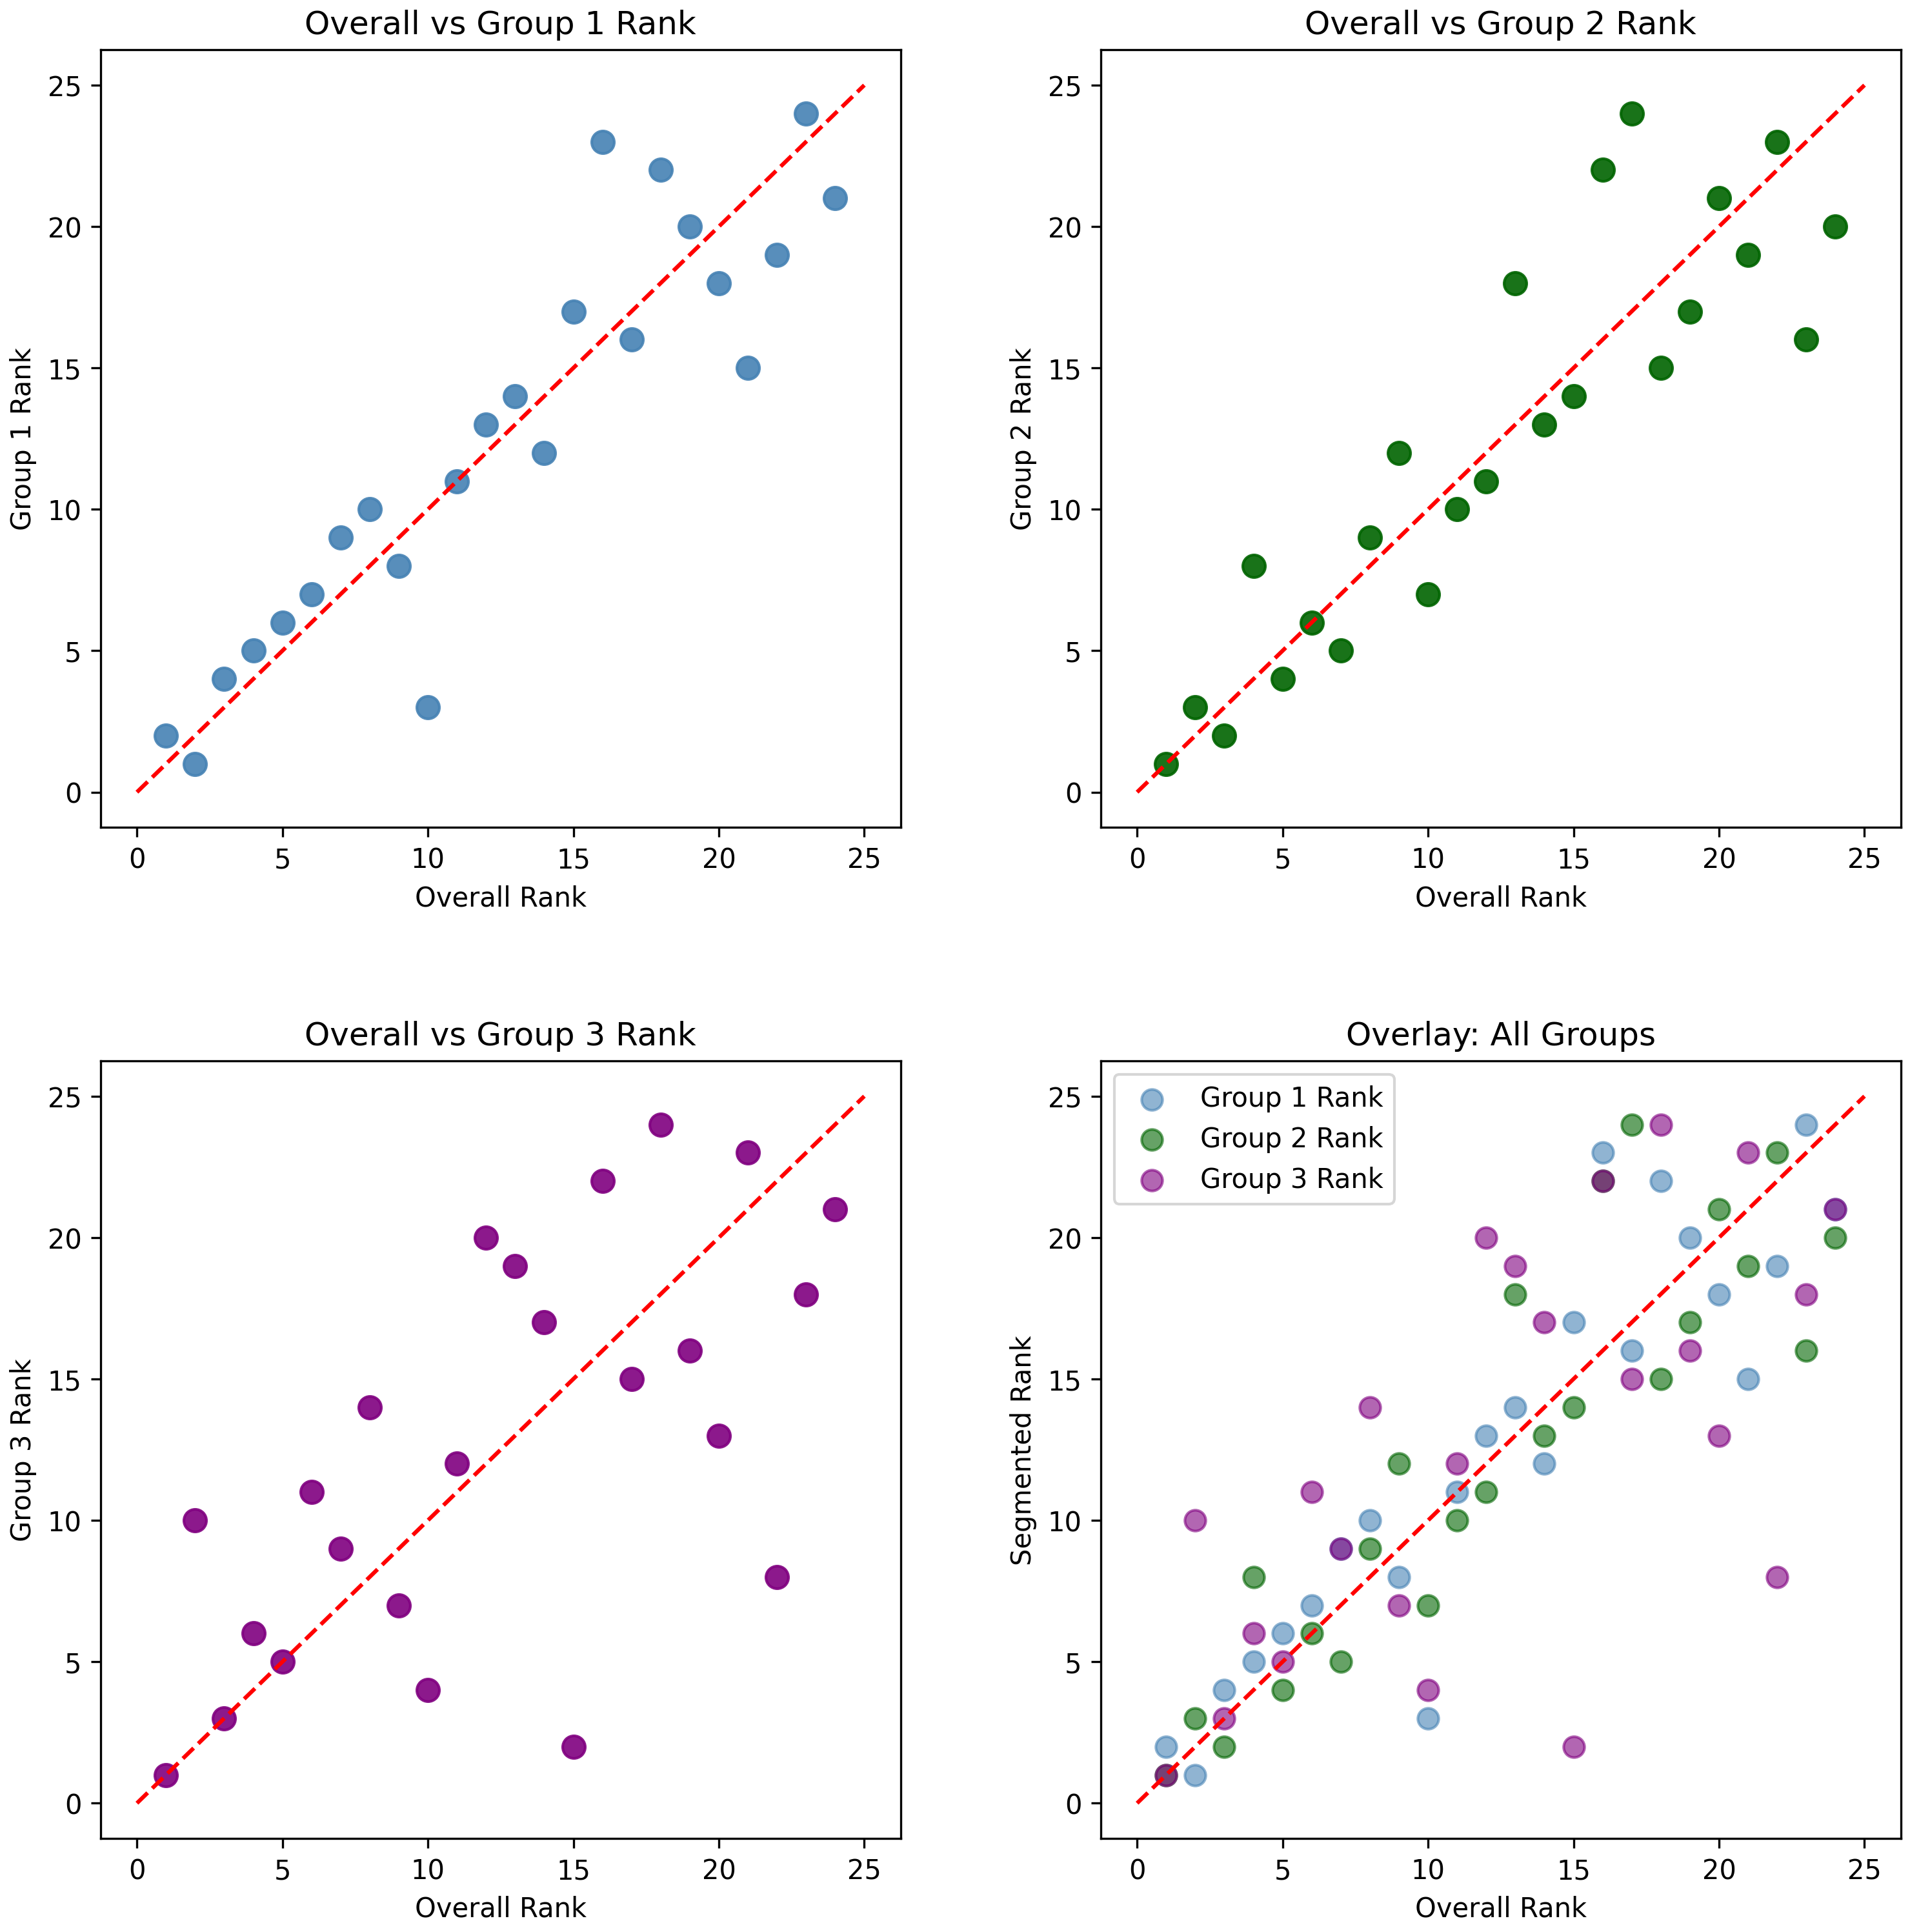
\includegraphics[width=0.9\textwidth]{feature_rank_overall_vs_groups_2x2_overlay.png}
\label{fig:overall-segmented-rank}
\end{figure}

\hypertarget{conclusion-and-discussion}{%
\section{6. Conclusion and Discussion}\label{conclusion-and-discussion}}

\hypertarget{interpretation-and-implications}{%
\subsection{6.1 Interpretation and
Implications}\label{interpretation-and-implications}}

This study examines which linguistic features are most strongly
associated with engagement in Yelp restaurant reviews. Because the
feature set was designed to capture interpretable aspects of
writing---lexical diversity, readability, syntactic structure, and
formatting---the models allow us to assess how these linguistic
indicators relate to engagement within the constraints of the dataset.
Logistic Regression provides linear, monotonic contributions, while
XGBoost captures nonlinear associations and interactions among
correlated features.

For features with roughly monotonic behavior---unique lemmas,
punctuation count, and syntactic depth---the two models produce similar
directional patterns. For features with more complex structure, such as
character count, the linear model compresses the marginal effect,
whereas XGBoost reflects nonlinear associations and plateaus. These
differences stem from the representational capacities of the models
rather than differences in the underlying linguistic signals.

The temporal segmentation analysis shows that the two earlier groups
reproduce the feature‑ranking patterns observed in the full dataset.
Group\,3 displays greater variability, likely reflecting incomplete
engagement accumulation or shifts in review composition. Even with this
noise, the segment‑specific rankings retain partial alignment with the
overall pattern, indicating that the main linguistic associations
persist across the temporal subsets examined.

Overall, the results show that vocabulary diversity, punctuation use,
and syntactic depth are consistently associated with higher engagement
in this dataset across modeling approaches and time periods. These
patterns help clarify how linguistic structure relates to engagement
signals in user‑generated content and may assist platforms in
identifying reviews that merit additional visibility when direct
engagement signals are sparse.

\hypertarget{limitations-and-future-directions}{%
\subsection{6.2 Limitations and Future
Directions}\label{limitations-and-future-directions}}

Several factors constrain how the findings should be interpreted and
point to directions for future work. These considerations help build a
fuller picture of how linguistic structure relates to engagement in
user‑generated content.

\begin{itemize}
\item
  \textbf{Domain restriction} - The study focuses on restaurant reviews
  to maintain a consistent writing domain. This improves internal
  validity but limits external validity. Applying the same methods to
  other Yelp categories or platforms would show whether the linguistic
  patterns generalize.
\item
  \textbf{Temporal incompleteness} - Newer reviews have had less time to
  receive votes, which reduces comparability across review age. Temporal
  segmentation in this study shows that key feature‑importance patterns
  remain stable in older periods, but fixed measurement windows or
  longitudinal designs would further reduce exposure‑time bias. These
  approaches may require platform‑level data access that is not publicly
  available.
\item
  \textbf{Contextual confounding} - Reviewer and business
  characteristics can influence engagement independently of language.
  Adding controls for reviewer activity, business popularity, or review
  visibility would help determine whether the observed linguistic
  patterns persist after accounting for these factors.
\item
  \textbf{Linguistic coverage} --- The current feature set captures core
  linguistic signals but not higher‑order writing structure. Embeddings
  and discourse‑level features were excluded for interpretability, but
  future work could incorporate them in a secondary analysis to provide
  a more complete representation of review language.
\end{itemize}

These limitations highlight opportunities to strengthen
interpretability, improve temporal comparability, and broaden the
linguistic and domain scope of engagement modeling.

\hypertarget{appendix}{%
\section{Appendix}\label{appendix}}

\hypertarget{a.1-data-availability}{%
\subsection{A.1 Data Availability}\label{a.1-data-availability}}

The analysis uses the publicly available Yelp Open Dataset. No
proprietary or restricted data were used.

\hypertarget{a.2-reproducibility-details}{%
\subsection{A.2 Reproducibility
Details}\label{a.2-reproducibility-details}}

All preprocessing, feature extraction, and modeling were implemented in
Python using the following library versions:\\
- spaCy 3.8.14 --- tokenization, POS tagging, lemmatization, dependency
parsing\\
- textstat 0.7.3 --- readability metrics\\
- vaderSentiment 3.3.2 --- sentiment scoring\\
- XGBoost 3.1.3 --- gradient‑boosted tree modeling\\
- scikit-learn 1.7.2 --- Logistic Regression and train--test splitting\\
- pandas 2.3.3 --- data manipulation\\
- Python 3.12.10 --- execution environment

All experiments were run on a standard consumer laptop (CPU‑only).

\hypertarget{references}{%
\section{References}\label{references}}

{[}1{]} Kim, S., Pantel, P., Chklovski, T., \& Pennacchiotti, M. (2006).
Automatically assessing review helpfulness. \emph{Proceedings of the
Conference on Empirical Methods in Natural Language Processing (EMNLP)}.

{[}2{]} Jindal, N., \& Liu, B. (2008). Opinion spam and analysis.
\emph{Proceedings of the ACM International Conference on Web Search and
Data Mining (WSDM)}.

{[}3{]} Mihalcea, R., \& Strapparava, C. (2009). The lie detector:
Explorations in the automatic recognition of deceptive language.
\emph{Proceedings of ACL‑IJCNLP}.

{[}4{]} Ghose, A., \& Ipeirotis, P. (2011). Estimating the helpfulness
and economic impact of product reviews: Mining text and reviewer
characteristics. IEEE Transactions on Knowledge and Data Engineering.

{[}5{]} Ott, M., Choi, Y., Cardie, C., \& Hancock, J. T. (2011). Finding
deceptive opinion spam by any stretch of the imagination.
\emph{Proceedings of the Association for Computational Linguistics
(ACL)}.

{[}6{]} Feng, S., Banerjee, R., \& Choi, Y. (2012). Syntactic stylometry
for deception detection. \emph{Proceedings of the Association for
Computational Linguistics (ACL)}.

{[}7{]} Mukherjee, A., Venkataraman, V., Liu, B., \& Glance, N. (2013).
What Yelp fake review filter might be doing? \emph{Proceedings of the
AAAI International Conference on Web and Social Media (ICWSM)}.

{[}8{]} Lundberg, S. M., \& Lee, S.-I. (2017). A unified approach to
interpreting model predictions. \emph{Proceedings of the 31st
International Conference on Neural Information Processing Systems
(NeurIPS)}.

{[}9{]} Qu, X., Li, X., Farkas, C., \& Rose, J. (2020). An attention
model of customer expectation to improve review helpfulness prediction.
\emph{In Advances in Information Retrieval (ECIR 2020), Lecture Notes in
Computer Science, 12035}

{[}10{]} Du, J., Rong, J., Wang, H., \& Zhang, Y. (2021). Neighbor‑aware
review helpfulness prediction. \emph{Decision Support Systems, 148}.

{[}11{]} Saumya, S., \& Kumar, P. (2023). Review helpfulness prediction
on e‑commerce websites: A comprehensive survey. \emph{Engineering
Applications of Artificial Intelligence, 126}.

\end{document}
